\begin{frame}{Multitask SACAAR}
    \begin{figure}
        \begin{minipage}[t]{0.45\linewidth}
            \centering
            \vspace{0pt}
            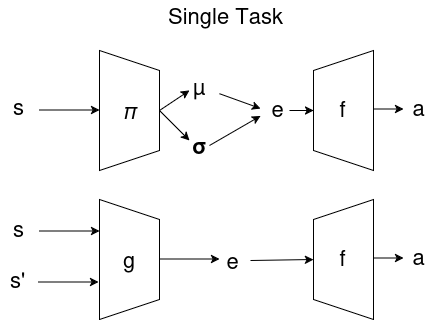
\includegraphics[width=\textwidth]{img/single_task_sacaar.png}
        \end{minipage}
        \hspace{0.5cm}
        \begin{minipage}[t]{0.45\linewidth}
            \centering
            \vspace{0pt}
            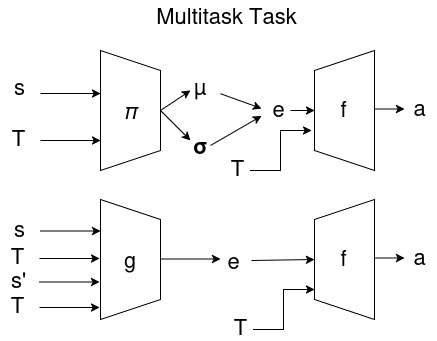
\includegraphics[width=\textwidth]{img/multi_task_sacaar.png}
        \end{minipage}
    \end{figure}
\end{frame}
\begin{frame}{Ànalise do vector condicionante de tarefa}
    \begin{figure}
        \centering
        \vspace{0pt}
        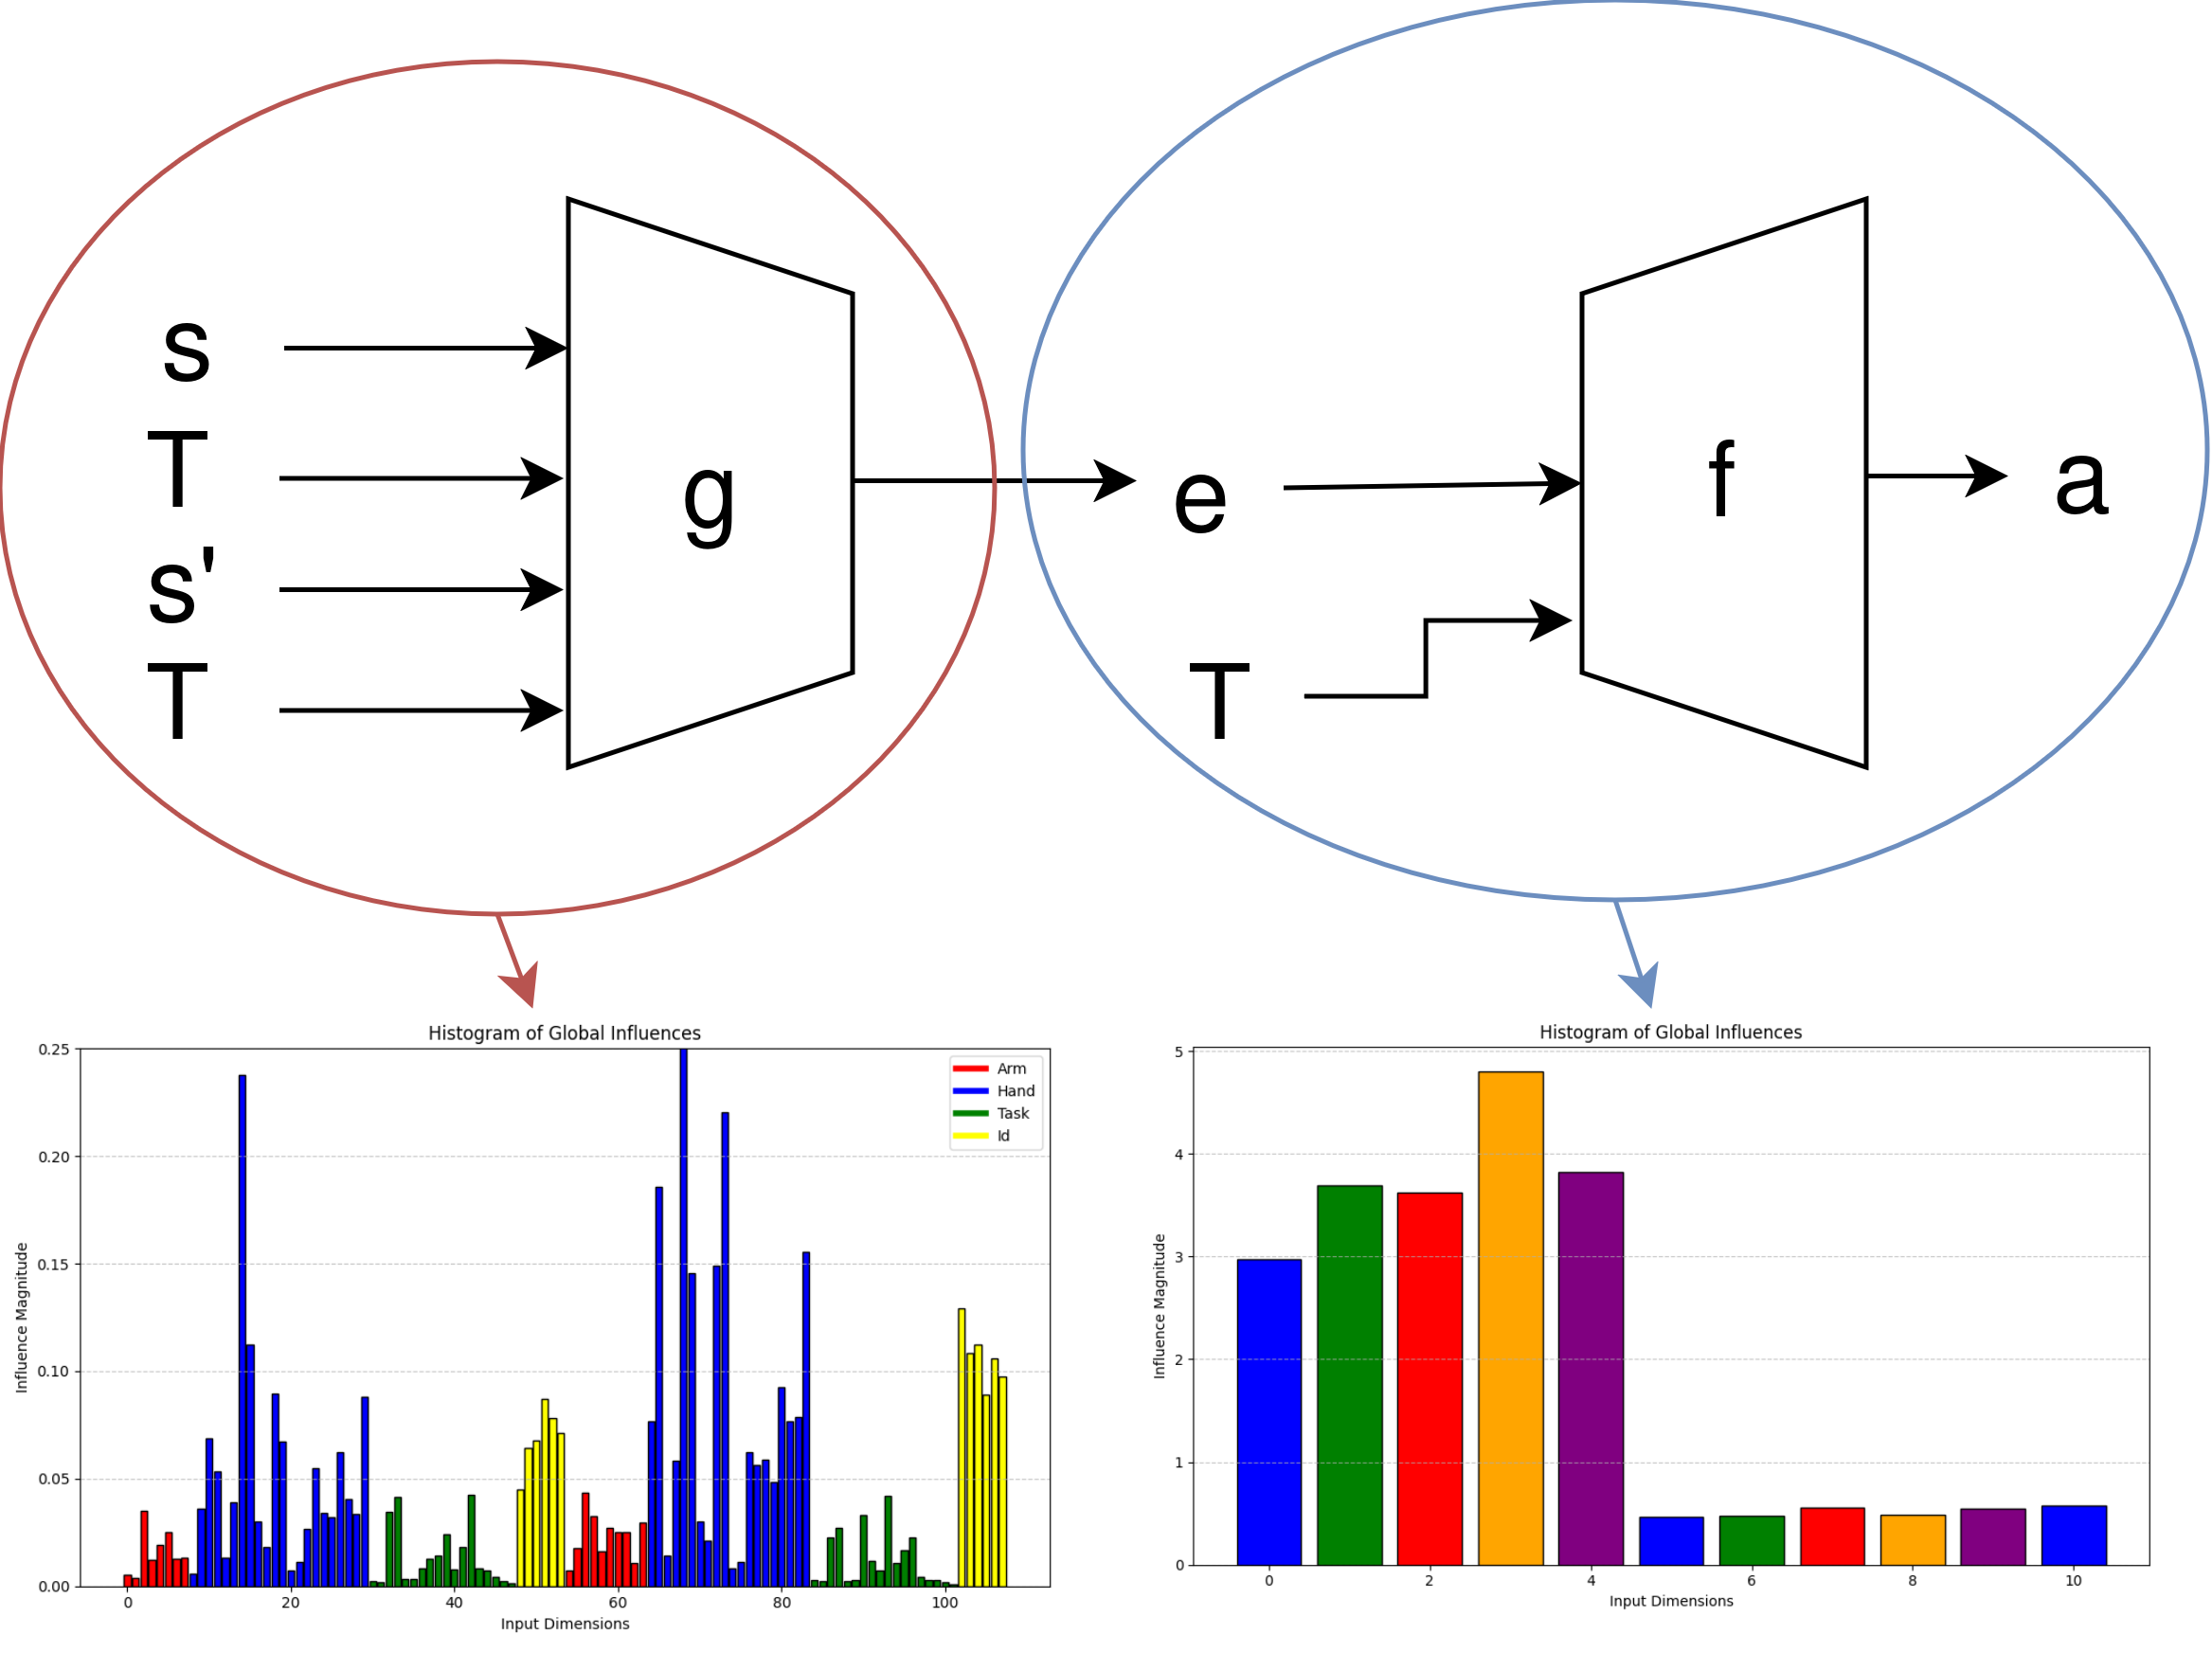
\includegraphics[width=0.7\textwidth]{img/sacaar_ig.png}
    \end{figure}
\end{frame}
\begin{frame}{Potenciais problemas}
    \begin{figure}
        \begin{minipage}[t]{0.4\linewidth}
            \centering
            \vspace{0pt}
            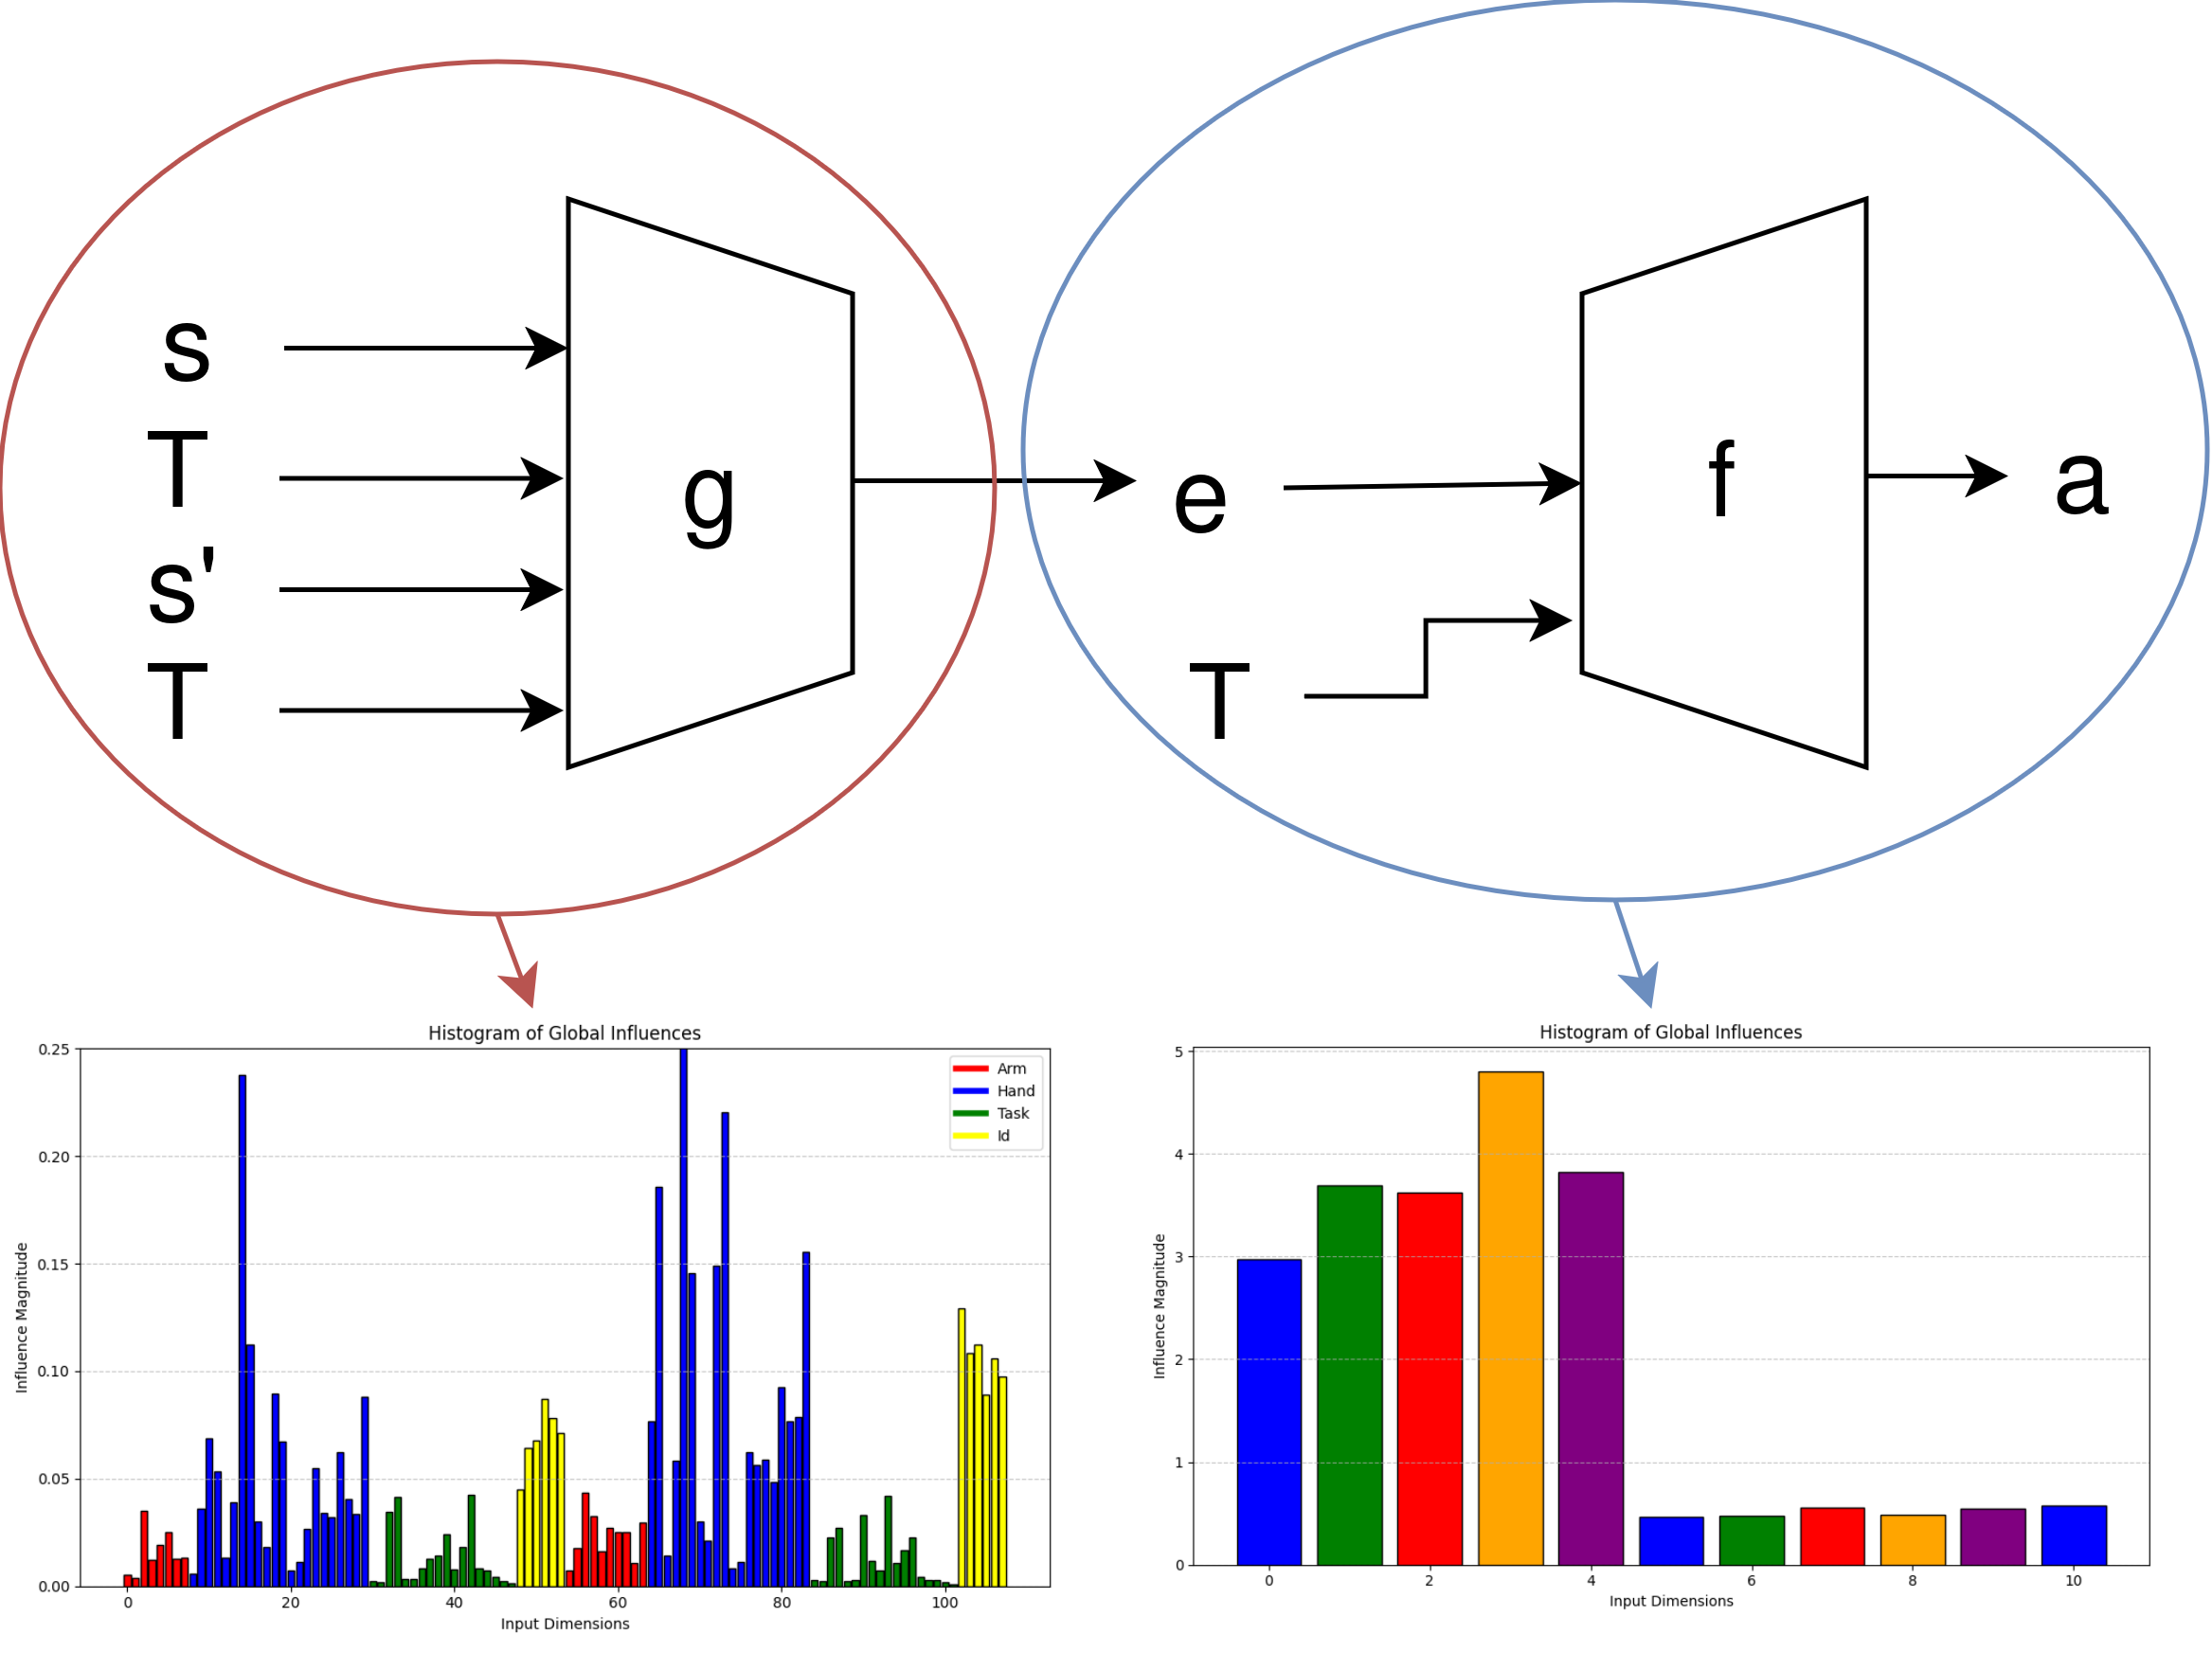
\includegraphics[width=\textwidth]{img/sacaar_ig.png}
        \end{minipage}
        \hspace{0.5cm}
        \begin{minipage}[t]{0.4\linewidth}
            \begin{itemize}
                \item Codificação one-hot (e.g. [1, 0, 0]) é demasiado esparsa.
                \item Informação da tarefa vem do input do encoder e é ignorada no condicionamento
                \item As ações no dataset são independente das ações
            \end{itemize}
        \end{minipage}
    \end{figure}
\end{frame}
\begin{frame}{Problema 1}
    Problema: Codificação one-hot (e.g. [1, 0, 0]) é demasiado esparsa.

    Solução: Utilizar um modelo que adquirir um vector de tarefa com valor mais continuo 

    \begin{figure}
        \begin{minipage}[t]{0.45\linewidth}
            \centering
            \vspace{0pt}
            
\includegraphics[width=\textwidth]{img/task_encoder.png}
        \end{minipage}
        \hspace{0.5cm}
        \begin{minipage}[t]{0.45\linewidth}
            \centering
            \vspace{0pt}
            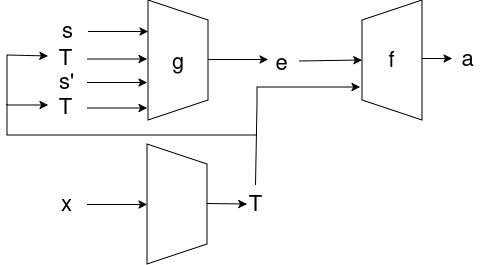
\includegraphics[width=\textwidth]{img/sacaar_encoded.png}
        \end{minipage}
    \end{figure}
\end{frame}
\begin{frame}{Problema 2}
    Problema: Informação da tarefa vem do input do encoder e é ignorada no condicionamento.

    Solução: Retirar a informação da tarefa do input do modelo de representação 

    \begin{figure}
        \centering
        \vspace{-10pt}
        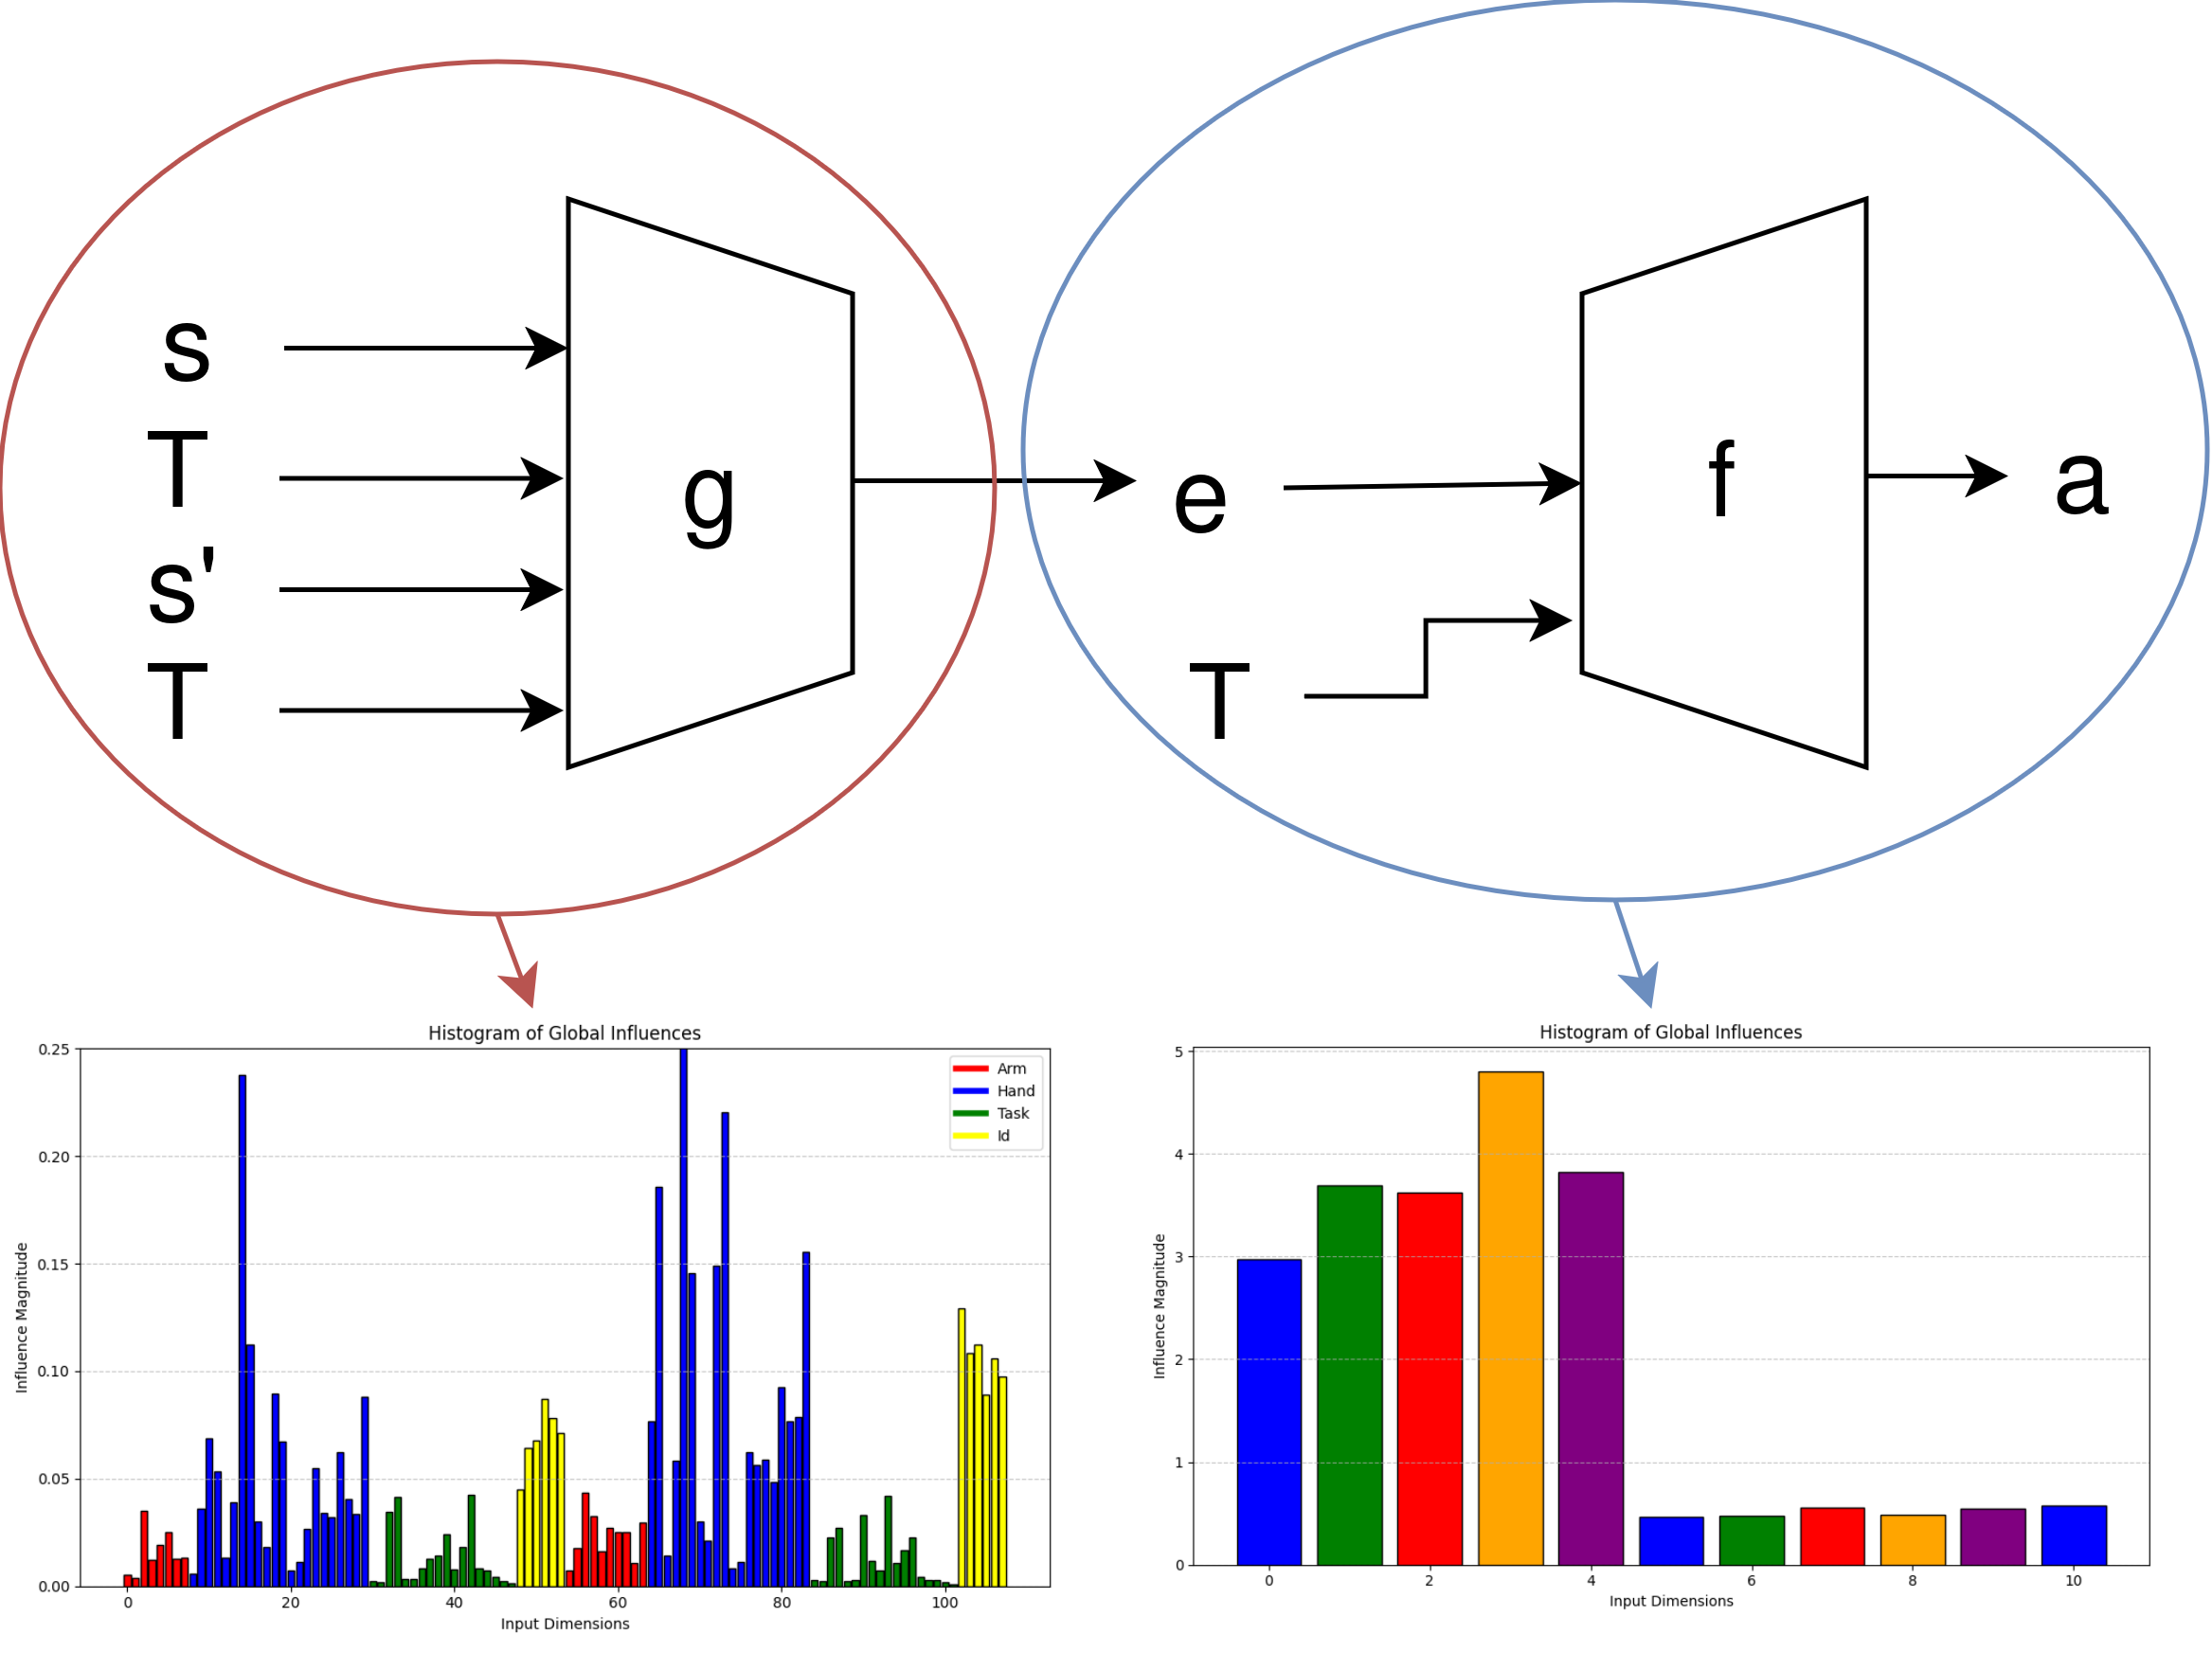
\includegraphics[width=0.8\textwidth]{img/sacaar_ig.png}
    \end{figure}
\end{frame}
\begin{frame}{Problema 3}
    Problema: As ações no dataset são independente das ações. O problema de exploração do SACAAR

    Solução: Melhorar a exploração permitindo sampling de ações fora da manifold. 

    \begin{figure}
        \begin{minipage}[t]{0.45\linewidth}
            \centering
            \vspace{0pt}
            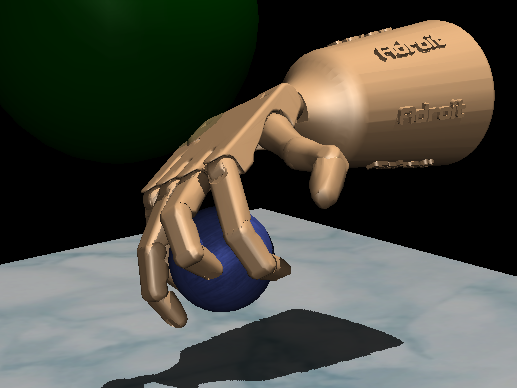
\includegraphics[width=\textwidth]{img/sphere.png}
        \end{minipage}
        \hspace{0.5cm}
        \begin{minipage}[t]{0.45\linewidth}
            \centering
            \vspace{0pt}
            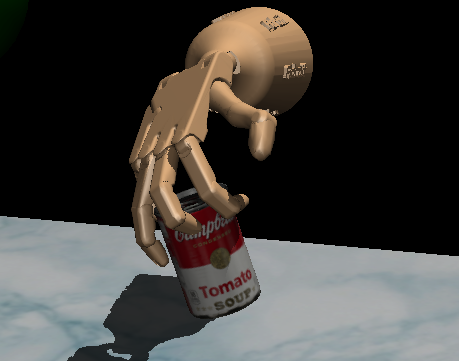
\includegraphics[width=\textwidth]{img/can.png}
        \end{minipage}
    \end{figure}
\end{frame}
\begin{frame}{Problema 3}
    Problema: As ações no dataset são independente das ações. O problema de exploração do SACAAR

    Solução: Melhorar a exploração permitindo sampling de ações fora da manifold. 

    \begin{figure}
        \centering
        \vspace{0pt}
        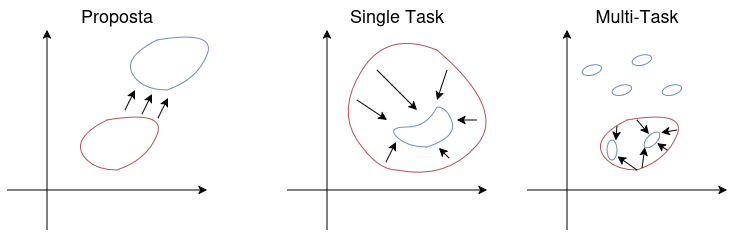
\includegraphics[width=\textwidth]{img/sacaar_exp.png}
    \end{figure}
\end{frame}
\begin{frame}{Problema 3}
    Problema: As ações no dataset são independente das ações. O problema de exploração do SACAAR

    Solução: Melhorar a exploração permitindo sampling de ações fora da manifold. 

    \begin{figure}
        \centering
        \vspace{0pt}
        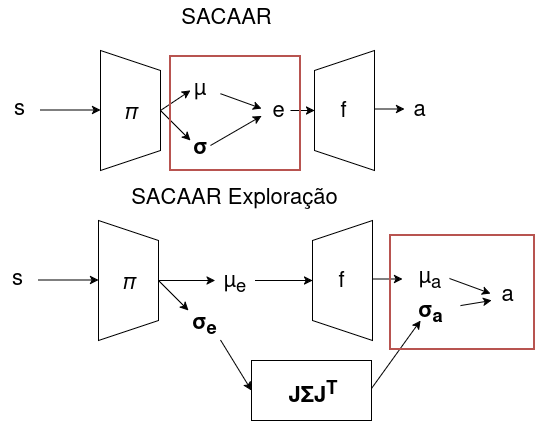
\includegraphics[width=0.65\textwidth]{img/sacaar_sigma.png}
    \end{figure}
\end{frame}
\begin{frame}{Problema 3}
    Problema: As ações no dataset são independente das ações. O problema de exploração do SACAAR

    Solução: Melhorar a exploração permitindo sampling de ações fora da manifold. 
    \begin{figure}
        \centering
        \vspace{-10pt}
        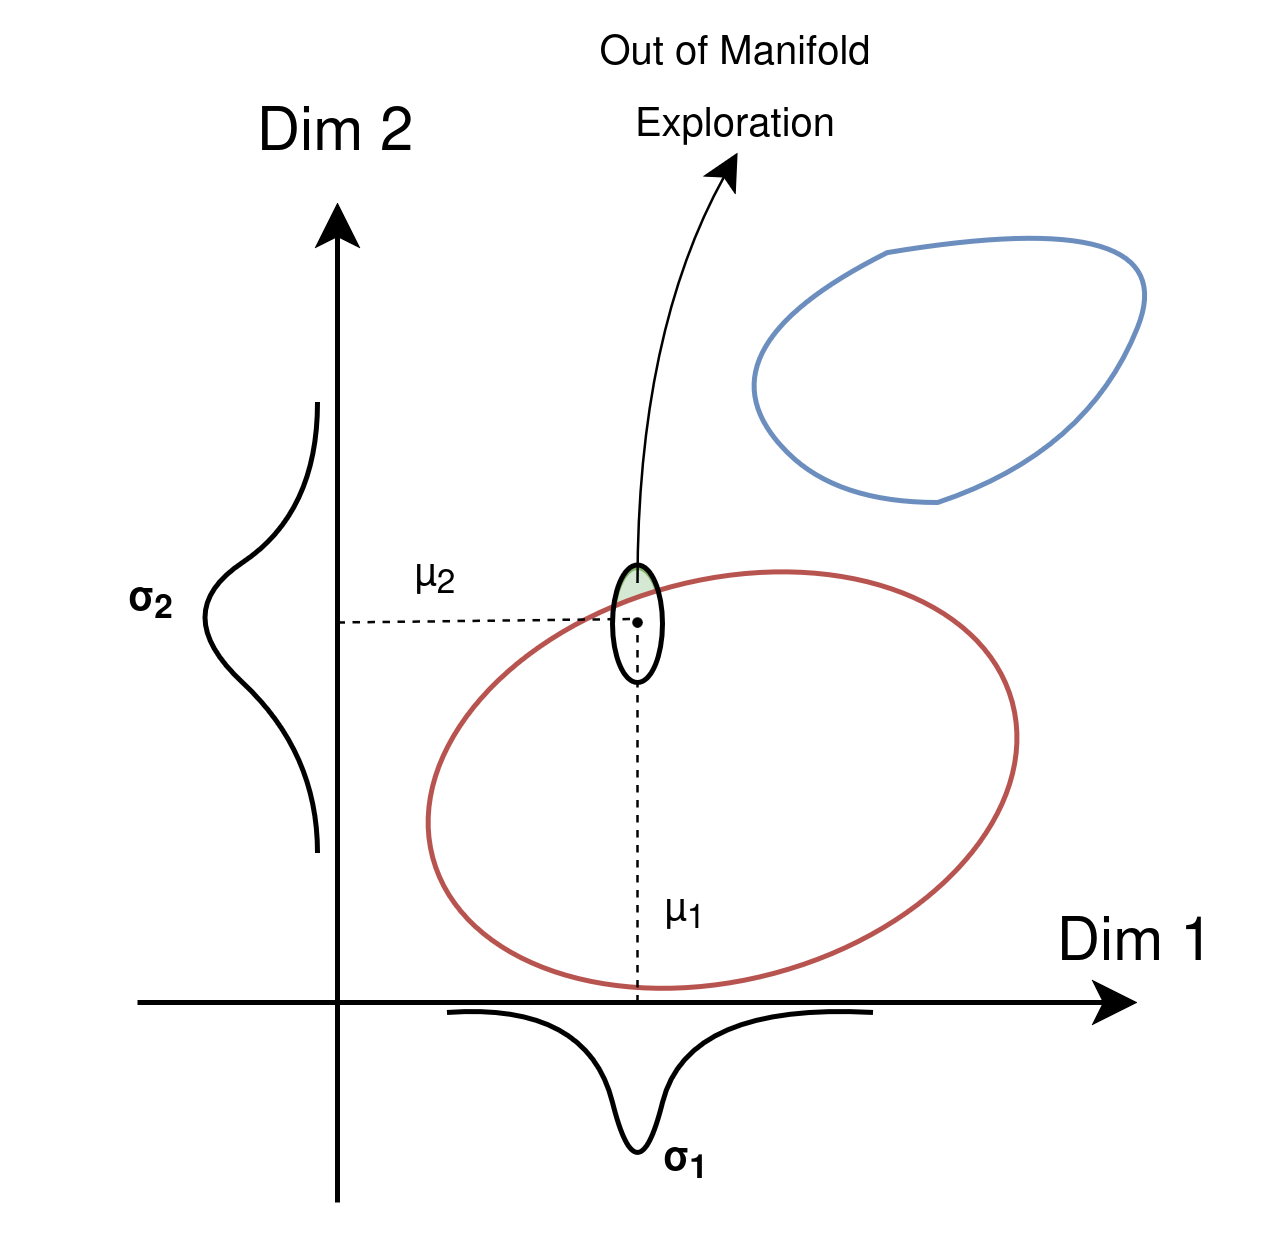
\includegraphics[width=0.6\textwidth]{img/sacaar_exp_man.png}
    \end{figure}
\end{frame}